\chapter{Fundamentação teórica}\label{ch:theory}

\section{O desafio da identificação digital}\label{section:desafio}

A prática de identificar pessoas para a prestação de serviços é muito comum e se manifesta em diversos contextos, desde o check-in de embarque até a recepção em estabelecimentos de saúde, onde são solicitados a apresentar documentos que confirmem sua identidade. Essa abordagem tornou-se imperativa para assegurar que as empresas possam aperfeiçoar a qualidade dos serviços oferecidos aos clientes, proporcionando uma experiência mais segura e personalizada. De maneira análoga, a identificação na web viabilizou um ambiente digital mais interativo e adaptado às preferências individuais. A exibição de telas com sugestões de produtos em uma loja eletrônica ou a orientação sobre quais perfis seguir em uma rede social são apenas alguns exemplos dentre a infinidade de possibilidades desse processo de personalização.
 
No entanto, esse procedimento suscita preocupações substanciais no que diz respeito à privacidade dos indivíduos. O monitoramento constante das ações dos usuários, muitas vezes conduzido de forma despercebida, pode resultar em uma intrusão significativa em suas vidas pessoais, minando a confiança essencial na relação entre eles e as plataformas digitais. Além disso, o compartilhamento não autorizado desses dados com terceiros representa uma ameaça significativa à segurança e à integridade das informações pessoais. A falta de controle sobre para quem e como esses dados são repassados pode conduzir a uma série de consequências prejudiciais, incluindo o seu potencial uso indevido, vazamento de informações sensíveis e até mesmo a manipulação de dados para fins maliciosos.

Nesse contexto, o avanço contínuo dos modelos de identidade na área de \acs{IAM} é impulsionado pela necessidade de abordar essas preocupações e encontrar soluções inovadoras. À medida que a tecnologia evolui, surgem métodos cada vez mais sofisticados e seguros para autenticação e autorização. Entre as abordagens exploradas estão as Provas de Conhecimento Zero, ou \sigla{ZKP}{Zero-Knowledge Proofs}, e a tecnologia blockchain, que visam equilibrar a segurança com a proteção da privacidade do usuário. As Provas de Conhecimento Zero constituem uma técnica criptográfica que permite verificar a veracidade de uma informação sem necessidade de revelá-la, preservando a privacidade dos dados. Já a blockchain funciona como uma estrutura de dados distribuída que registra informações de forma transparente e imutável, garantindo a integridade e rastreabilidade dos dados sem recorrer a uma autoridade central. Dessa maneira, o desenvolvimento de modelos de identidade mais robustos busca não apenas aprimorar a segurança, mas também oferecer uma experiência digital personalizada, preservando a confidencialidade e a integridade das informações pessoais.

\section{Modelos de Identidades}\label{section:modelos}

Modelo de identidade refere-se a uma representação abstrata que descreve como as identidades são gerenciadas, autenticadas e autorizadas em um sistema de computação. A identidade, predominantemente representada por meio de uma \textbf{credencial} contendo afirmações acerca do usuário, conhecidas por \textbf{claims}, e são de importância crucial para o controle de acesso e a segurança em ambientes computacionais. Essa representação possibilita a determinação de quais entidades possuem permissão para acessar recursos específicos e realizar ações designadas. Portanto, os modelos de identidade são estruturados em entidades que desempenham papéis específicos ao longo do ciclo de vida da credencial \cite{bertino2009identity}. Essas entidades incluem:

\begin{itemize}
    
    \item \textbf{Usuário:} Representa o indivíduo interessado em utilizar um serviço. No entanto, o acesso a esse serviço requer a sua identificação.
    
    \item \textbf{\acs{SP}}: Entidade que solicita a identificação do usuário para permitir o acesso aos seus serviços.
    
    \item \textbf{\acs{IdP}}: Responsável por emitir credenciais (identificação) para os usuários que desejam acessar algum serviço.
    
\end{itemize}

Os modelos são categorizados em três tipos distintos \cite{revisao-ssi-frederico}: centralizado, terceirizado e auto-soberano. Cada uma dessas classificações representa uma abordagem única em termos de interação e organização dos elementos mencionados anteriormente. A  \autoref{fig:identity-models} oferece uma representação visual de cada modelo respectivamente, os quais serão detalhadamente descritos nas próximas subseções.

% % Figura com os três modelos de identidade
\begin{figure}[htb]
    \caption{Modelos de identidade.}
    \centering
    \resizebox{\linewidth}{!}{
        \begin{tabular}{c c c}
            % Modelo Centralizado
\begin{minipage}[b]{0.4\linewidth}
    \centering
    \begin{tikzpicture}[roundnode/.style={circle, draw=black, very thick, minimum size=20mm, align=center},]
        %Nodes
        \node[roundnode]      (idp-sp)                            {IdP \\ SP};
        \node[roundnode]      (usr)  [left=of idp-sp]  {usuário};
        
        %Lines
        \draw[<->] (idp-sp) -- (usr);

    \end{tikzpicture}
\end{minipage} & 
            % Modelo Terceirizado
\begin{minipage}[b]{0.5\linewidth}
    \centering
    \begin{tikzpicture}[roundnode/.style={circle, draw=black, very thick, minimum size=20mm},]
        %Nodes
        \node[roundnode]      (idp)                            {IdP};
        \node[roundnode]      (sp)     [below right=of idp]  {SP};
        \node[roundnode]      (usr)    [below left=of idp]   {usuário};
        
        %Lines
        \draw[<->] (idp) -- (usr);
        \draw[<->]  (usr) -- (sp);
        % Linha paralela e traçada
        \draw[->, dashed] (sp) edge[bend right=5, draw=none] coordinate[at start](sp-b) coordinate[at end](idp-b) (idp)
                  edge[bend left=5, draw=none] coordinate[at start](sp-t) coordinate[at end](idp-t) (idp)
              (sp-t) -- (idp-t);

        \draw[<->] (idp-b) -- (sp-b);
    
    \end{tikzpicture}
\end{minipage} & 
            
% Modelo Centralizado
\begin{minipage}[b]{0.5\linewidth}
    \centering
    \begin{tikzpicture}[roundnode/.style={circle, draw=black, very thick, minimum size=20mm, align=center},]
        %Nodes
        \node[roundnode]      (idp)                            {IdP};
        \node[roundnode]      (sp)     [below right=of idp]  {SP};
        \node[roundnode]      (usr)    [below left=of idp]   {usuário\\IdP};
        
        %Lines
        \draw[<->] (idp) -- (usr);
        \draw[<->]  (usr) -- (sp);
        \draw[->, dashed] (sp) edge[bend right=5, draw=none] coordinate[at start](sp-b) coordinate[at end](idp-b) (idp)
                  edge[bend left=5, draw=none] coordinate[at start](sp-t) coordinate[at end](idp-t) (idp)
              (sp-t) -- (idp-t);
        \draw[->, dashed] (sp) edge[bend right=5, draw=none] coordinate[at start](sp-b) coordinate[at end](usr-b) (usr)
                  edge[bend left=5, draw=none] coordinate[at start](sp-t) coordinate[at end](usr-t) (usr)
              (sp-t) -- (usr-t);
    
    \end{tikzpicture}
\end{minipage} \\ \\
            (a) Modelo Centralizado & (b) Modelo Terceirizado & (c) Modelo SSI
        \end{tabular}
    }
    \vspace{0.5cm}
    \fonte{\citeonline{revisao-ssi-frederico}}
    \label{fig:identity-models}
\end{figure}


\subsection{Centralizado}\label{subsection:centralizado}

Na década de 1960, a internet ainda estava em seus primórdios, e poucos serviços web estavam disponíveis. Nessa época, era comum que cada site mantivesse seu próprio sistema interno para gerenciar as credenciais dos usuários, desempenhando simultaneamente as funções de \acs{SP} e \acs{IdP}. Assim, cada sistema decidia quais informações eram necessárias para identificar o usuário em seu contexto específico, enquanto os próprios usuários eram responsáveis por administrar suas credenciais, mantendo uma senha única para cada aplicativo que utilizavam \cite{wangham2008gerenciamento}. 

No final dos anos 1990 e início dos anos 2000, uma série de serviços e plataformas surgiram, tornando a internet mais atrativa. Entre eles estavam os serviços de e-mail como Yahoo Mail e Hotmail, os motores de busca como Google, o comércio eletrônico com Amazon e eBay, e as redes sociais, começando com MySpace e seguido pelo Facebook em 2004. Essa explosão de novos serviços resultou em um aumento significativo no número de credenciais que as pessoas precisavam gerenciar. Como consequência, muitos optaram por senhas mais simples e fáceis de lembrar, ou até mesmo começaram a reutilizar senhas entre diferentes serviços \cite{evernym2024}. Essa prática comprometeu consideravelmente a segurança das informações pessoais, pois a violação de apenas uma senha poderia permitir acesso a vários aspectos da vida digital.

Além disso, esse modelo enfrentou desafios ao tentar oferecer uma melhor experiência de navegação ao usuário. Cada aplicação da época tinha seu próprio procedimento para a criação de credenciais de acesso, o que levava muitas pessoas a preencherem os formulários de maneira incompleta ou incorreta, na tentativa de obter acesso ao serviço o mais rapidamente possível. Isso prejudicava a capacidade de personalização da experiência, impactando negativamente na apresentação de conteúdos e funcionalidades adaptadas às preferências e necessidades individuais \cite{wangham2008gerenciamento}.

Para superar as dificuldades do modelo centralizado, um novo paradigma foi proposto e foi possível melhorar a experiência do usuário, reduzir a carga administrativa de múltiplas credenciais e aumentar a segurança dos dados pessoais. Ele ficou conhecido como modelo terceirizado.

\subsection{Terceirizado}\label{subsection:terceirizado}

A proliferação de provedores de serviços destacou de forma evidente os problemas previamente descritos. Gerenciar uma senha para cada plataforma acessada tornou-se um ônus significativo para os indivíduos, enquanto que, para os desenvolvedores, representava uma sobrecarga substancial. Isso se devia à necessidade de alocar recursos consideráveis para a manutenção e segurança das credenciais em seus sistemas. A solução para esse problema foi terceirizar essa responsabilidade para uma nova entidade, o \acs{IdP}, levando esse modelo a ser conhecido por modelo terceirizado \cite{revisao-ssi-frederico}. Nesse sentido, diversos protocolos foram criados para padronizar as interações entre \acs{IdP}, \acs{SP} e usuários finais, como os protocolos de troca de tokens, como OAuth 2.0 \cite{oauth} e OpenID Connect \cite{openid}.

Além disso, começou a ser utilizado o conceito de autenticação única, conhecido como \sigla{SSO}{Single Sign-On}. O \acs{SSO} permite que os indivíduos façam login uma única vez para acessar múltiplos provedores de serviços, sem a necessidade de se autenticar novamente em cada um deles, até que as credenciais expirem. Esse avanço significativo simplificou consideravelmente a experiência do usuário, tornando o processo de autenticação mais eficiente e conveniente. Com o \acs{SSO}, o compartilhamento de identidades entre diferentes provedores de serviços tornou-se mais fluido, aumentando a usabilidade e a satisfação do usuário.

Além de melhorar a experiência do usuário, o \acs{SSO} também proporciona benefícios adicionais, como a redução da fadiga de senha, já que os indivíduos não precisam lembrar de múltiplas senhas para diferentes serviços. Isso, por sua vez, pode melhorar a segurança, pois os eles são menos propensos a utilizar senhas fracas ou repetidas em diferentes plataformas. No entanto, é crucial garantir a segurança das credenciais de \acs{SSO}, pois o comprometimento de uma única conta pode potencialmente dar acesso a múltiplos serviços.

Apesar dos progressos alcançados, é importante destacar algumas desvantagens relacionadas à privacidade. O risco se concentra na possibilidade de que os dados pessoais coletados durante o processo de verificação de identidade e compartilhamento de informações sejam comprometidos ou divulgados de maneira inadequada, ou ainda, mal utilizados por uma das partes que têm acesso a eles, tipicamente \acs{IdP} e \acs{SP} \cite{pandey2012investigation}. Sobre a prerrogativa de oferecer melhores serviços, fazer melhorias e personalizar a experiência, muitos \acs{IdP}s, como o Google \cite{sidell2020google}, coletam dados sobre a forma como usuário usa seus dispositivos, apps e serviços, incluindo o comportamento de navegação.


\subsection{Auto-Soberano}\label{subsection:auto-soberano}

O modelo Auto-Soberano é um paradigma de gestão de identidades que tem se destacado nos últimos anos com o avanço das tecnologias de armazenamento de dados descentralizados, como blockchains. Nesse modelo, o controle das informações pessoais é transferido para os indivíduos, permitindo-lhes determinar com quem, quando e de que maneira compartilham seus dados \cite{bosch2024selfsovereign}. Em contraste com os modelos tradicionais, nos quais os dados são geridos por entidades centralizadas, o modelo Auto-Soberano proporciona maior privacidade e autonomia ao usuário, pois elimina intermediários e centraliza a gestão de identidade no próprio indivíduo.

No contexto da \acs{SSI}, o modelo de Credenciais Verificáveis, conforme proposto pela W3C \cite{data-model-w3c}, é amplamente adotado. Esse modelo faz uso das \textbf{\sigla{VC}{Verifiable Credentials}}, também chamadas por Credencias Verificáveis, que são documentos digitais emitidos pelo \acs{IdP} e contêm informações específicas sobre o indivíduo que podem ser verificadas criptograficamente por qualquer entidade. Além disso, o titular das credenciais tem a capacidade de gerar \textbf{\sigla{VP}{Verifiable Presentation}}, ou em português Apresentações Verificávies, que são estruturas para a apresentação de dados de identidade digital, codificadas de modo a garantir que a autoria das informações seja verificável criptograficamente, assegurando assim sua autenticidade e integridade sem a necessidade de revelar informações adicionais além do necessário.

As \acs{VP}s utilizam duas técnicas principais para minimizar a exposição de informações sensíveis: \textbf{Divulgação Seletiva} e \textbf{\acs{ZKP}}. A Divulgação Seletiva permite ao titular compartilhar apenas partes específicas dos dados contidos nas credenciais, restringindo a divulgação ao mínimo necessário para a verificação, enquanto o restante dos dados permanece protegido. Essa abordagem proporciona um controle granular sobre quais informações são reveladas, fortalecendo a privacidade e a segurança. Por exemplo, em uma \acs{VC} que contenha nome, data de nascimento e endereço, o titular pode optar por compartilhar apenas o nome e omitir os demais detalhes. A Prova de Zero-Conhecimento é outra técnica poderosa empregada nas \acs{VP}s, o qual é possível provar a veracidade de uma afirmação sem revelar os dados subjacentes. Por exemplo, pode-se demonstrar que uma pessoa é maior de idade sem expor sua data de nascimento específica. Este conceito será explorado mais detalhadamente na \autoref{section:zkp}.

O fluxo de \acs{VC}s e \acs{VP}s entre os atores \acs{IdP}, Usuário e \acs{SP} está representado na  (\autoref{fig:vc-data-model}). O processo inicia-se com o \acs{IdP}, que desempenha o papel de entidade responsável pela criação e emissão da \acs{VC}. O \acs{IdP} gera a credencial associada a um identificador.  Normalmente, um \textbf{identificador} é usado para obter uma chave pública criptográfica, necessária para verificar a assinatura digital na credencial. As opção mais conhecida para identificador são os certificados X.509, mas também há outros exemplos como \sigla{DID}{Identificador Descentralizado} que utilizam um Registro de Dados Verificáveis para obter a chave. A associação é feita pela assinatura é fundamental para assegurar tanto a autenticidade quanto a integridade da credencial, garantindo que qualquer entidade verificadora possa, posteriormente, confirmar que a credencial foi emitida por uma fonte legítima e que não sofreu alterações.
 
Após a emissão, a \acs{VC} é entregue ao titular, que a armazena em uma carteira digital. Esta carteira digital, cuja funcionalidade será detalhada na \autoref{subsection:carteira-digital}, é um progrma2 específico destinado ao armazenamento seguro das credenciais. Quando o \acs{SP} exige que determinada informação seja compartilhada ou provada, ele solicita a apresentação de um \acs{VP} correspondente. O titular, então, gera e compartilha a \acs{VP} de maneira segura por meio da carteira digital. Utilizando o identificador, o titular recupera a chave pública e com a assinatura anexada à \acs{VP}, o \acs{SP} pode verificar instantaneamente a autenticidade e a integridade da credencial apresentada.

\begin{figure}[htb]
    \caption{Modelo de Credenciais Verificáveis W3C}
    \centering
    \resizebox{0.7\linewidth}{!}{
        \begin{tikzpicture}[
  >={Stealth[round]},
  every node/.style={align=center},
  IdP/.style={draw, rounded corners, fill=gray!30, minimum height=2em, minimum width=3cm},
  usr/.style={draw, rounded corners, fill=gray!30, minimum height=2em, minimum width=4cm},
  sp/.style={draw, rounded corners, fill=gray!30, minimum height=2em, minimum width=3cm},
  registry/.style={draw, rounded corners, fill=gray!30, minimum height=3em, minimum width=5cm},
  line/.style={-Stealth, thick, black},
  node distance=2cm and 3cm, % Adjust node distance for spacing
]

    % Nodes
    \node[IdP] (IdP) {\acs{IdP}\\(Website)};
    \node[usr, right=of IdP] (usr) {Usuário\\(Carteira Digital)};
    \node[sp, right=of usr] (sp) {\acs{SP}\\(Website)};
    \node[registry, below=of usr, yshift=-1cm] (registry) {Registro de Dados Verificáveis}; % Adjusted position
    
    % Arrows
    \draw[line] (IdP) -- node[above] {Emissão\\de\\\acs{VC}s} (usr);
    \draw[line] (usr) -- node[above] {Submissão\\de\\\acs{VP}s} (sp);
    \draw[line] (IdP) -- node[sloped, above] {Utiliza\\\acs{VC}s} (registry);
    \draw[line] (usr) -- node[sloped, below] {Utiliza\\\acs{VC}s} (registry);
    \draw[line] (sp) --  node[sloped, above]  {Verifica\\\acs{VP}s} (registry);
    
\end{tikzpicture}

    }
    \fonte{O Autor}
    \label{fig:vc-data-model}
\end{figure}

Contudo, a adoção deste modelo exige que os usuários adotem uma postura mais proativa e participativa na gestão de suas informações pessoais. Essa necessidade de envolvimento direto pode representar um desafio significativo, especialmente para o público leigo que utiliza ambientes digitais sem grande preocupação com as complexidades subjacentes de segurança \cite{revisao-ssi-frederico}. A situação é análoga aos desafios enfrentados pelo \sigla{PGP}{Pretty Good Privacy}, uma tecnologia de criptografia desenvolvida nos anos 1990 para garantir a segurança e privacidade de e-mails e arquivos. O \acs{PGP} utiliza um sistema de criptografia de chave pública, permitindo que os usuários troquem informações de forma segura. No entanto, apesar de ser uma ferramenta poderosa, o \acs{PGP} enfrentou dificuldades de adoção devido à complexidade envolvida na configuração e gestão segura dos pares de chaves, o que limitou seu uso entre o público geral \cite{allen2016}. O gerenciamento adequado de chaves públicas e privadas é tecnicamente exigente e requer um nível de conhecimento que muitos usuários não possuem, o que pode limitar a adoção ampla de sistemas baseados no modelo Auto-Soberano.


\subsubsection{Carteiras Digitais}\label{subsection:carteira-digital}

Carteiras digitais surgem no âmbito da \acs{IAM} com propósitos variados, adaptados a diferentes modelos de uso. De maneira geral, uma carteira digital é um programa que armazena informações de identidade digital, permitindo que usuários gerenciem suas credenciais e realizem transações seguras online \cite{digital_identity_wallet_benefits_and_risks}. 

Com as carteiras digitais, é possível obter o armazenamento seguro para material criptográfico associado aos dados de identidade digital, como chaves de assinatura criptográficas. O usuário consegue controlar e gerenciar suas informações, incluindo remover e revisar os dados armazenados na carteira, além de selecionar explicitamente quais dados deseja armazenar ou compartilhar, tanto dentro quanto fora da carteira. \cite{podgorelec2024digital}. Além disso, as carteiras digitais também são caracterizadas por sua acessibilidade, sendo utilizáveis através de dispositivos móveis, como smartphones e tablets. Elas frequentemente suportam múltiplas formas de autenticação, incluindo senhas, biometria (como impressão digital e reconhecimento facial) e autenticação multifator \cite{future_of_digital_wallets_and_identity_management}.

Portanto, as carteiras digitais representam uma evolução significativa na forma como as identidades digitais são gerenciadas e protegidas, promovendo a descentralização e conferindo maior controle individual sobre dados pessoais. Nesse modelo, o próprio usuário mantém o controle de suas informações, sem depender de uma entidade central para gerenciar ou armazenar seus dados. Assim, a identidade digital é centralizada apenas para o usuário, enquanto o gerenciamento de identidade como um todo se torna mais descentralizado no ecossistema digital.


\subsubsection{Prova de Zero Conhecimento}\label{section:zkp}

Prova de Zero Conhecimento (\acs{ZKP}) trata-se de um método no qual uma parte, denominada provador, é capaz de demonstrar a outra parte, denominada verificador, a veracidade de uma determinada afirmação, sem revelar qualquer informação adicional além da própria afirmação em questão \cite{petkus2019zkSNARK}. Esse esquema de prova é utilizado de forma ampla em criptomoedas, como ZCash, para garantir a privacidade, e também nos sistemas de identidade digital para realizar a autenticação sem revelar informações de maneira excessiva.

Para garantir a privacidade e a segurança das informações dos usuários em sistemas de identidade digital, existem diferentes tipos de prova que podem ser utilizadas para permitir que os detentores de identidade provem certos atributos de suas credenciais sem revelar os dados completos, como a de igualdade, desigualdade e prova de pertencimento a um conjunto \cite{Sovrin_ZKP}. A prova de igualdade é usada para mostrar que um atributo é igual a um valor específico, como provar que está empregado apenas com uma resposta de afirmação ou negação. A prova de desigualdade demonstra que um atributo numérico está dentro de um certo intervalo sem revelar o valor exato, como provar que uma pessoa possui mais de 21 anos sem informar a idade exata. A prova de pertencimento a um conjunto confirma que um atributo pertence a um grupo específico sem revelar o valor exato, como mostrar que alguém reside em um país europeu sem dizer qual país. Essas técnicas aumentam a confiança e a segurança ao permitir que os usuários compartilhem informações verificáveis sem expor dados sensíveis desnecessariamente.

Nessa perspectiva esse esquema de prova abre um caminho para uma redução significativamente do risco de ataques de phishing e engenharia social, bem como o vazamento de dados. Isso ocorre porque as \acs{ZKP}s permitem que os usuários verifiquem suas identidades ou atributos sem revelar informações sensíveis durante o processo de autenticação \cite{Farias2024ZKP}. Como as informações secretas nunca são compartilhadas, mesmo em interações com terceiros, os atacantes não têm acesso a dados críticos que poderiam ser usados para fraudes ou ataques direcionados. Esse nível de privacidade e segurança impede que dados confidenciais sejam interceptados ou manipulados, mitigando efetivamente os riscos associados a esses tipos de ameaças.

\subsubsubsection*{Fundamentos e Funcionamento}

 As \acs{ZKP}s baseiam-se em três propriedades fundamentais: completude, solidez e zero-conhecimento. A completude assegura que, se uma declaração é verdadeira, o verificador aceitará o resultado da prova. A solidez garante que, se a declaração for falsa, o provador não conseguirá criar uma prova falsa para enganar o verificador. Por fim, a propriedade de zero-conhecimento assegura que o verificador não obtém nenhuma informação adicional sobre o provador além do que está explicitamente contido na prova. O processo geral envolve quatro etapas principais: autenticação, troca de provas, verificação e conclusão \cite{Farias2024ZKP}.

\begin{enumerate}

    \item Autenticação: O provador (quem detém a informação) e o verificador (quem precisa confirmar a veracidade) estabelecem um canal de comunicação seguro. O provador prepara a prova baseada na informação que deseja validar.

    \item Troca de provas: O provador gera uma prova criptográfica e a envia ao verificador. Esta prova é estruturada de forma que demonstre a veracidade da declaração sem revelar a própria informação.

    \item Verificação: O verificador analisa a prova recebida utilizando um algoritmo que confirma se a prova é válida. Esse processo assegura que a prova é consistente com a declaração sem necessitar de acesso à informação subjacente.

    \item Conclusão: Se a prova é validada, o verificador aceita a declaração como verdadeira. Caso contrário, a declaração é rejeitada. Importante notar que o verificador não adquire conhecimento adicional sobre a informação que o provador está protegendo.
    
\end{enumerate}
    

Essas etapas garantem a segurança e a privacidade das informações, pois o verificador pode confiar na autenticidade da declaração sem comprometer a confidencialidade dos dados.

\subsubsubsection*{Protocolos Existentes}

Os protocolos \acs{ZKP}s são amplamente utilizados em diversas aplicações, especialmente em cenários onde a privacidade e a segurança são essenciais. Existem dois tipos de protocolos, sendo estes classificados como interativos ou não interativos. Nos protocolos interativos, a verificação envolve uma série de interações dinâmicas entre o provador e o verificador. Durante esse processo, o verificador faz uma série de desafios, e o provador responde a cada um deles em tempo real, provando passo a passo o conhecimento da informação sem revelá-la. Em contraste, os protocolos não-interativos permitem que o provador prepare uma prova completa e independente, que pode ser verificada posteriormente por qualquer verificador, sem necessidade de interação adicional. Esses protocolos geralmente dependem do uso de funções de hash para gerar provas verificáveis sem interação contínua \cite{petkus2019zkSNARK}.

O exemplo de protocolo não-interativo mais conhecido é o \sigla{ZK-SNARK}{Zero-Knowledge Succinct Non-Interactive Arguments of Knowledge} \cite{Farias2024ZKP} devido à sua capacidade de executar provas extremamente compactas. Por essa razão, são considerados ideais para adoção em sistemas com restrições de armazenamento e largura de banda limitadas.

Atualmente, algumas bibliotecas e ferramentas facilitam a implantação do \acs{ZK-SNARK} de maneira prática e eficiente em sistemas reais. Essas bibliotecas permitem que desenvolvedores utilizem \acs{ZKP}s sem precisar de um conhecimento profundo da criptografia subjacente, tornando a tecnologia mais acessível. As mais famosas são: snarkjs e circom. A snarkjs é uma biblioteca JavaScript para a criação e verificação de \acs{ZK-SNARK}, enquanto a circom é uma linguagem específica de domínio, \sigla{DSL}{Domain Specific Language}, projetada para descrever circuitos aritméticos utilizados nos \acs{ZK-SNARK} \cite{belles2023circom}. 

A principal desvantagem dos ZK-SNARKs é a necessidade de uma configuração inicial confiável, \textit{trusted setup}. Durante essa fase, um conjunto inicial de parâmetros públicos, chamado \sigla{CRS}{Common Reference String}, é gerado. A segurança de todo o sistema depende da integridade desse processo. Se o \acs{CRS} for comprometido, por exemplo, ou se os dados temporários (resíduos tóxicos) gerados durante a configuração não forem destruídos corretamente, uma entidade maliciosa poderia criar provas falsas e enganar o sistema.

Nesse sentido, os protocolos \sigla{ZK-STARK}{Zero-Knowledge Scalable Transparent ARguments of Knowledge}  são uma variante mais recente, projetada para superar algumas limitações dos \acs{ZK-SNARK}, especialmente em termos de transparência e escalabilidade. Considerados resistentes aos ataques de computadores quânticos. Esses argumentos são muito úteis em contextos onde os conceitos de transparência e escalabilidade são críticos, além de possuírem destaque na aplicabilidade e eficiência \cite{Farias2024ZKP}. No entanto, as bibliotecas atuais para a implementação de \acs{ZK-STARK} em sistemas reais não são tão fáceis e intuitivas, especialmente quando comparadas às bibliotecas snarkjs e circom, que oferecem um nível mais elevado de abstração e facilidade de uso para \acs{ZK-SNARK}. Essa complexidade adicional  representa um desafio significativo para os desenvolvedores que desejam implementar \acs{ZK-STARK} de maneira eficaz.

\subsection{Fiduciário}\label{subsection:fiduciário}

O quarto e último modelo a ser apresentado representa um conjunto de esforços destinados a superar as limitações observadas nos modelos anteriores. Conhecido como Fiduciário, esse novo paradigma busca encontrar uma solução para a dicotomia entre a experiência do usuário durante os procedimentos de autenticação e manipulação de dados, e o fortalecimento da preservação da privacidade desses dados. Enquanto sistemas de gerenciamento de identidades baseados em modelos terceirizados oferecem uma experiência de navegação satisfatória, facilitada pelos mecanismos de \acs{SSO}, eles enfrentam dificuldades em evitar a divulgação desnecessária de dados em certos contextos. Em contrapartida, as propostas existentes de \acs{SSI} conseguem solucionar esse problema, mas apresentam uma experiência de usuário insatisfatória \cite{fiduciary}, com interações complexas e demoradas com os provedores de serviços e as carteiras.

O modelo fiduciário propõe que a gestão das identidades do usuário deve ser realizada por um novo agente de confiança, conhecido como fiduciário. Este, por sua vez, estabelece um relacionamento que dá origem a seu nome, fiduciário, que estabelece uma relação de confiança e responsabilidade em que uma parte (o fiduciário) tem o dever legal e ético de agir no melhor interesse da outra parte (o beneficiário). Esse tipo de relacionamento é comum em várias áreas, como no direito, na administração de empresas, saúde e na gestão de investimentos, e é ilustrado na \autoref{fig:fiduciary-model} através das linhas duplas tracejadas. Este modelo também se caracteriza por inúmeras características de segurança e usabilidade, porém elas podem agrupadas nos seguintes princípios fundamentais: \emph{Consent by Default}, \emph{Transparency for Accountability} e \emph{Non-Disclosure as a Goal}.

\begin{figure}[htb]
    \caption{Pilares do Modelo Fiduciário}
    \centering
    \resizebox{\linewidth}{!}{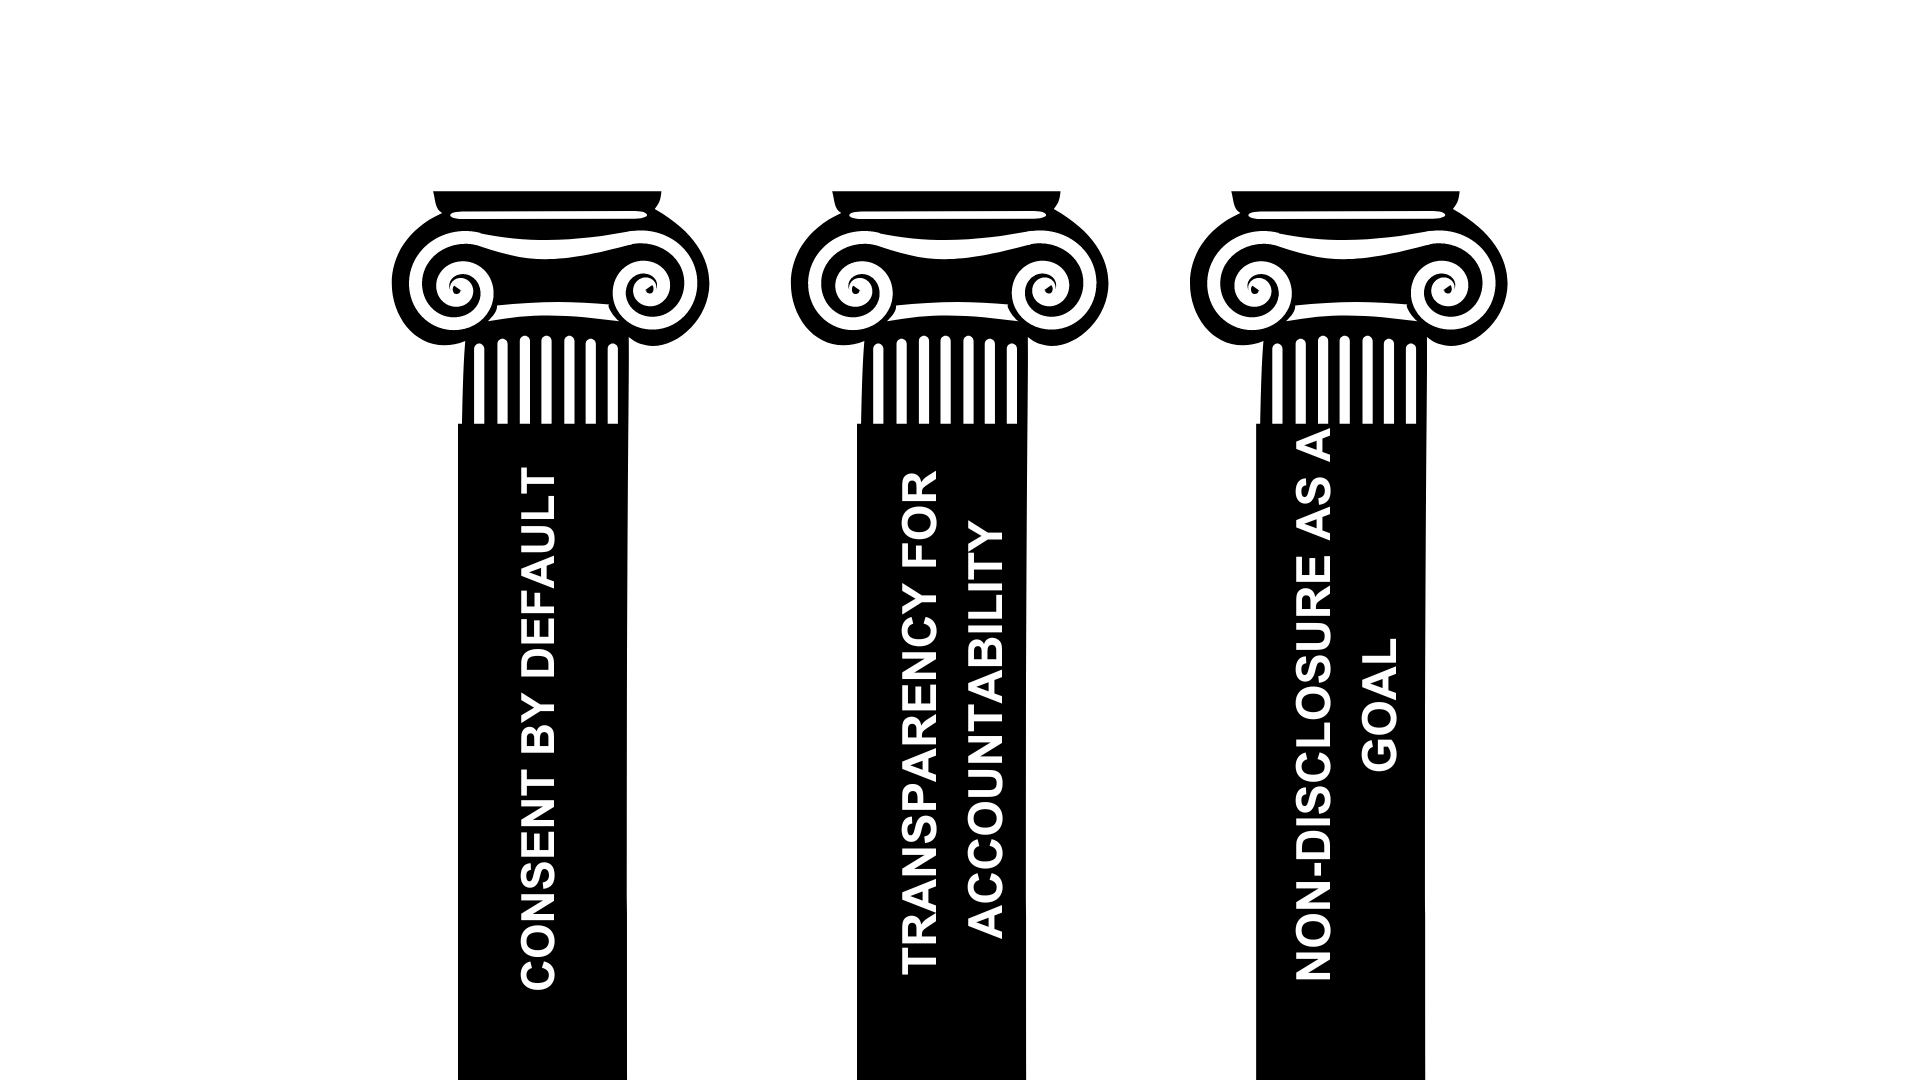
\includegraphics{images/png/pilares-do-FIM.png}}
    \fonte{O Autor}
    \label{fig:princilpes}
\end{figure}


O primeiro princípio, \emph{Consent by Default}, dita que todas as ações do fiduciário devem ser guiadas pelos consentimentos que o indivíduo definiu. Isso é implementado por meio de um artefato computacional chamado Política de Consentimento, que estabelece um conjunto de declarações feitas pelo usuário que definem o que pode ser feito com seus dados em termos de coleta, armazenamento e compartilhamento com outras entidades. Por meio deste artefato, o Fiduciário consegue decidir quais credenciais são mais adequadas para serem usadas em determinados contextos, seguindo a orientação do que o titular considera sensível sobre seus dados, possibilitando que ele não perca o controle sobre sua identidade digital. Essa política pode ser definida previamente, antes que as interações entre o usuário e \acs{SP} ocorram, ou sob demanda, caso o Fiduciário não consiga determinar claramente se sua ação pode ou não prejudicar a pessoa.

À primeira vista, a introdução de uma nova entidade responsável pelo gerenciamento dos dados pode parecer um retrocesso, retirando o controle dos indivíduos sobre suas próprias credenciais. Contudo, o objetivo é proporcionar suporte àqueles que enfrentam dificuldades ou preferem não se preocupar com as exigências de segurança relacionadas à manutenção de credenciais. As Políticas de Consentimento são projetadas para garantir que os titulares dos dados tenham todo o controle desejado, permitindo que flexibilizem ou restrinjam as ações do Fiduciário. Dessa forma, o Fiduciário pode atuar tanto como uma carteira digital presente nos modelos de \acs{SSI} quanto como um elo de confiança, ciente de suas responsabilidades e deveres, capacitado a tomar as melhores decisões em benefício do dono dos dados.

O segundo princípio, \emph{Transparency for Accountability}, estabelece que deve ser viável rastrear de forma precisa as ações realizadas sobre determinados dados, especificando o momento em que ocorreram e para quais finalidades foram utilizadas. Para esse propósito, é definido um artefato computacional denominado \emph{Evidências}, que serve para auditar toda e qualquer atividade realizada pelo fiduciário com os dados dos utilizadores. Através desse mecanismo, é possível realizar um processo sistemático de exame e avaliação das atividades e modificações de dados efetuadas pelo fiduciário, com o objetivo de verificar a conformidade com as políticas de consentimento e boas práticas, bem como avaliar a eficácia, eficiência e integridade dessas manipulações.

Ao permitir que o Fiduciário tome decisões de forma autônoma, ele pode se basear em solicitações anteriores semelhantes ou em outras métricas, visando reduzir as interrupções constantes aos usuários. Contudo, a autonomia conferida ao Fiduciário não o isenta de cometer erros na utilização dos dados dos indivíduos. Na prática, essa autonomia e os registros das ações garante ao beneficiário que seu representante será responsabilizado caso ocorra qualquer atitude delituosa. Adicionalmente, um aspecto significativo deste novo artefato é a sua capacidade de aprimorar a rastreabilidade das ações de um invasor que consiga comprometer o ambiente de execução do Fiduciário e conseguisse agir como tal agente. Isso se deve ao fato de que todas as atividades realizadas pelo Fiduciário serão registradas de forma detalhada, permitindo uma análise minuciosa e precisa das ações executadas durante a intrusão.

O terceiro princípio, \emph{Non-Disclosure as a Goal}, determina que o principal objetivo do modelo é manter a confidencialidade e evitar a revelação de determinadas informações, seja na construção de novos protocolos ou interfaces que utilizam o modelo como estrutura. Para alcançar esse objetivo, três mecanismos podem ser empregados: Divulgação Seletiva, \acs{ZKP} (Prova de Conhecimento Zero) e Seleção de Ambiente de Execução. Embora cada um desses mecanismos possa ser aplicado individualmente, a combinação deles potencializa significativamente o grau de preservação das informações dos beneficiários.

A primeira estratégia fundamenta-se na capacidade do Fiduciário de revelar apenas partes específicas das informações do usuário, sem expor a totalidade de seus dados. Para alcançar esse objetivo, busca-se a utilização de \acs{VC} que disponibilizem mecanismos para a construção de \acs{VP} que contenham apenas um subconjunto de atributos, em vez de incluir todos os atributos disponíveis. A segunda estratégia é baseada na utilização de  \acs{ZKP}, conforme detalhado na \autoref{section:zkp}, pois apesar de também ser uma solução de divulgação seletiva, essa abordagem reduz de forma significativa a exposição de dados em comparação à seleção de atributos para uma \acs{VP}. Independentemente do mecanismo adotado, o modelo visa proporcionar ao indivíduo maior controle sobre seus dados pessoais, permitindo-lhe fornecer apenas as informações estritamente necessárias e, assim, minimizar a exposição de dados supérfluos ou potencialmente invasivos.

A terceira estratégia explora a possibilidade de processamento de dados fora do ambiente do \acs{SP}. Tradicionalmente, o processamento de dados relacionados à identidade ocorre em um ambiente de confiança controlado pelo \acs{SP}, sem oferecer ao usuário a opção de escolher o ambiente que considera mais seguro, resultando na transferência obrigatória de dados de um ambiente para outro. No entanto, o modelo proposto introduz duas alternativas: a primeira permite que o processamento ocorra em um ambiente de confiança do próprio titular dos dados, em consonância com a proposta de \citeonline{opal}. A segunda possibilita a computação colaborativa entre diferentes entidades por meio de técnicas seguras de Computação Multipartidária, conhecida em inglês como \sigla{MPC}{Multiparty Computation}, assegurando que os dados de cada participante permaneçam privados e confidenciais ao longo de todo o processo. 


% Figura do modelo Fiduciário (Conceitual)
\begin{figure}[htb]
    \caption{Modelo Fiduciário.}
    \centering
    \resizebox{0.8\linewidth}{!}{\begin{minipage}[b]{0.5\linewidth}
    \centering
    \begin{tikzpicture}[roundnode/.style={circle, draw=black, very thick, minimum size=20mm, align=center},]
        % Nodes
        \node[roundnode]      (idp)                            {IdP};
        \node[roundnode]      (sp)     [below right=3cm and 1cm of idp]  {SP}; % Adjusted positioning
        \node[roundnode]      (fid)    [below left=3cm and 1cm of idp]  {Fiduciário}; % Adjusted positioning
        \node[roundnode]      (usr)    [left=of fid]  {usuário};
        
        % Lines
        \draw[<->] (idp) -- (fid);
        \draw[<->]  (fid) -- (sp);
        \draw[->, dashed] (sp) edge[bend right=5, draw=none] coordinate[at start](sp-b) coordinate[at end](idp-b) (idp)
                  edge[bend left=5, draw=none] coordinate[at start](sp-t) coordinate[at end](idp-t) (idp)
              (sp-t) -- (idp-t);
        \draw[<->] (fid) edge[bend right=-5, draw=none] coordinate[at start](fid-b) coordinate[at end](usr-b)(usr)
              edge[bend left=-4, draw=none] coordinate[at start](fid-t) coordinate[at end](usr-t) (usr)
             (fid-t) -- (usr-t);
        \draw[<-, double, dashed] (usr) edge[bend right=5, draw=none] coordinate[at start](usr-b) coordinate[at end](fid-b) (fid)
              edge[bend left=-10, draw=none] coordinate[at start](usr-t) coordinate[at end](fid-t) (fid)
             (usr-t) -- (fid-t);
    \end{tikzpicture}
\end{minipage}
}
    \vspace{0.5cm}
    \fonte{Inspirado em \citeonline{revisao-ssi-frederico}}
    \label{fig:fiduciary-model}
\end{figure}

\section{Protocolos de Identidade Digital}\label{subsection:protocolos}

\subsection{OAuth 2.0}\label{subsubsection:oauth}

OAuth 2.0 é um protocolo  de autorização que fornece à aplicações a capacidade de acessar um recurso de usuário por meio de tokens, evitando que o indivíduo precise compartilhar a sua credencial de acesso com aplicação. Dessa forma, não há necessidade de compartilhar credenciais sensíveis \cite{oauth}. Por exemplo, um leitor pode autorizar um aplicativo de notícias à acessar sua conta ou realizar postagens em seu nome na sua conta de sua rede social sem revelar para o aplicativo qual é a senha. Caso o aplicativo de notícias sofra algum tipo de vazamento de dados, a senha da rede social desse leitor continua resguardada no \acs{IdP}, a rede social.

Para que o protocolo funcione adequadamente, quatro papéis principais são essenciais no processo. Primeiramente, temos o \textbf{Proprietário do recurso}, que corresponde ao indivíduo que deseja autorizar uma aplicação a acessar seus dados. No cenário ilustrativo de leitura de notícias, o Proprietário do recurso seria o leitor que pretende permitir que um aplicativo acesse suas preferências de leitura. Em segundo lugar, o \textbf{Cliente} é a aplicação que almeja utilizar os dados do indivíduo. Mantendo o exemplo anterior, o cliente seria o aplicativo de notícias que deseja acessar as preferências do leitor para personalizar o conteúdo apresentado. O terceiro papel é desempenhado pelo \textbf{Servidor de Autorização}, que é o responsável por autenticar o usuário e fornecer tokens que permitem ao cliente acessar os recursos do indivíduo. Este servidor atua como uma ponte de confiança entre o Proprietário do recurso e o cliente, assegurando que apenas aplicativos devidamente autorizados possam acessar os dados. Finalmente, temos o \textbf{Servidor de Recurso}, que é o servidor responsável por armazenar os dados do indivíduo. Frequentemente, o servidor de recurso coincide com o servidor de autorização, embora possam ser distintos dependendo da arquitetura do serviço implementado. Comparando com o modelo terceirizado da \autoref{fig:identity-models}, o Servidor de Autorização e o Servidor de Recurso correspondem ao \acs{IdP}, o Proprietário do recurso representa o Usuário, e o \acs{SP} é o Cliente.

Além desses papéis, o protocolo utiliza tokens, credenciais que representam a autorização, para gerenciar o acesso aos recursos. Alguns deles são \textbf{Código de Autorização}, \textbf{Token de Acesso} e o \textbf{Token de Atualização}. O Código de Autorização (Authorization Grant) é um token fornecido ao cliente após a autenticação do usuário perante o servidor de autorização. Este código é utilizado pelo cliente para obter um Token de Acesso e se trata de uma sequência de caracteres que comprova que o usuário autorizou o cliente a agir em seu nome. O Código de Acesso (Access Token) é o token que determina o tipo de acesso que o cliente terá sobre os recursos do indivíduo. Este token geralmente inclui informações sobre o escopo específico de acesso, o tempo de validade e outros atributos relevantes; no entanto, o provedor pode personalizar o conteúdo do token conforme suas necessidades. É com este token que o cliente realiza efetivamente o acesso aos dados. Por fim, os tokens de atualização (Refresh Tokens) permitem que a aplicação obtenha novos Tokens de Acesso sem a necessidade de reautenticação do usuário. O uso de Tokens de Atualização reduz a frequência com que o usuário precisa interagir com o processo de autenticação, melhorando a segurança, já que o usuário não precisa fornecer suas credenciais repetidamente.

O OAuth 2.0 utiliza o protocolo \sigla{HTTP}{HyperText Transfer Protocol} para transmitir parâmetros durante o processo de autorização. Quando um cliente inicia uma solicitação de autorização, ele redireciona o navegador do usuário para o Ser3vidor de Autorização utilizando o método \acs{HTTP} GET, incluindo alguns parâmetros na URL da requisição. Três parâmetros importantes nesse contexto são o \textbf{\texttt{\texttt{scope}}}, \textbf{\texttt{response\_type}} e \textbf{\texttt{client\_id}}. O parâmetro \texttt{scope} define o nível de acesso que o cliente está solicitando, especificando as permissões desejadas. Por exemplo, uma aplicação pode solicitar acesso apenas à leitura de emails ou à leitura e escrita de contatos. 

O parâmetro \texttt{response\_type} define o fluxo de mensagens para autenticação e autorização, determinando o tipo de resposta que o Cliente deve esperar do Servidor de Autorização. Existem quatro fluxos distintos: \textbf{Fluxo de Código de Autorização} (Authorization Code Flow), \textbf{Fluxo Implícito} (Implicit Flow), \textbf{Fluxo de Credenciais de Senha do Proprietário do Recurso} (Resource Owner Password Credentials Flow) e \textbf{Fluxo de Credenciais do Cliente} (Client Credential Flow). Assim, dependendo \texttt{response\_type} escolhido e outros parâmetros, algum desses fluxo poderá ser utilizado. Por exemplo, se o \texttt{response\_type} é \texttt{code}, utiliza-se o Fluxo de Código de Autorização, onde o cliente recebe um código de autorização que será trocado por um Token de Acesso. Já se for o \texttt{response\_type}=\texttt{token} é utilizado no Fluxo Implícito, onde o cliente recebe diretamente um Token de Acesso.

Outro parâmetro crucial é o \texttt{client\_id}, que identifica de forma única a aplicação cliente que está solicitando acesso aos recursos do usuário. Este identificador é fornecido pelo Servidor de Autorização quando a aplicação é registrada. Em combinação com o \texttt{client\_secre}t, que é um segredo conhecido apenas pela aplicação e pelo Servidor de Autorização, o \texttt{client\_id} ajuda a autenticar a aplicação durante o processo de obtenção do Token de Acesso. Além disso, as requisições ao servidor de autorização geralmente incluem a \texttt{redirect\_uri}, que é a URL para a qual o usuário será redirecionado após o processo de autenticação e autorização. Esta URL deve ser registrada previamente no Servidor de Autorização e corresponder exatamente ao que foi registrado para evitar ataques de redirecionamento malicioso.

Há também a definição de vários endpoints usados ao longo do processo de autorização. O \textbf{Authorization Endpoint} é o URL onde o usuário é redirecionado para fornecer o consentimento e autenticar. Este endpoint processa as solicitações de autorização e emite Códigos de Autorização ou tokens, dependendo do fluxo. O \textbf{Token Endpoint} é utilizado para trocar um Código de Autorização por um Token de Acesso, sendo também usado para renovar Tokens de Acesso expirados. O \textbf{Resource Endpoint} é onde os recursos protegidos são acessados. O cliente usa o Token de Acesso para solicitar recursos do servidor de recursos.

Esses papéis, artefatos, parâmetros e endpoints permitem construir uma implementação robusta do OAuth 2.0, assegurando acesso seguro e controlado a recursos, sem comprometer as credenciais dos usuários. O protocolo é flexível e adaptável, equilibrando segurança e usabilidade conforme as necessidades das aplicações.

A \autoref{fig:oauth}, descrita a seguir, demonstra o funcionamento do \emph{Fluxo de Código de Autorização}. Nesse fluxo, ocorre a obtenção de um \emph{Código de Autorização}, que é subsequentemente trocado por um Token de Acesso. Na figura, observa-se que, após o usuário selecionar o \acs{IdP} de sua preferência, como o Facebook, ele é redirecionado pelo navegador por meio de uma requisição realizada pelo \acs{SP} (Cliente). A partir desse ponto, o fluxo descrito na imagem é iniciado.
% Figura dos funcionamento do oauth
\begin{figure}[htb]
    \caption{Fluxo de Código de Autorização no OAuth}
    \centering
    
    \resizebox{0.8\linewidth}{!}{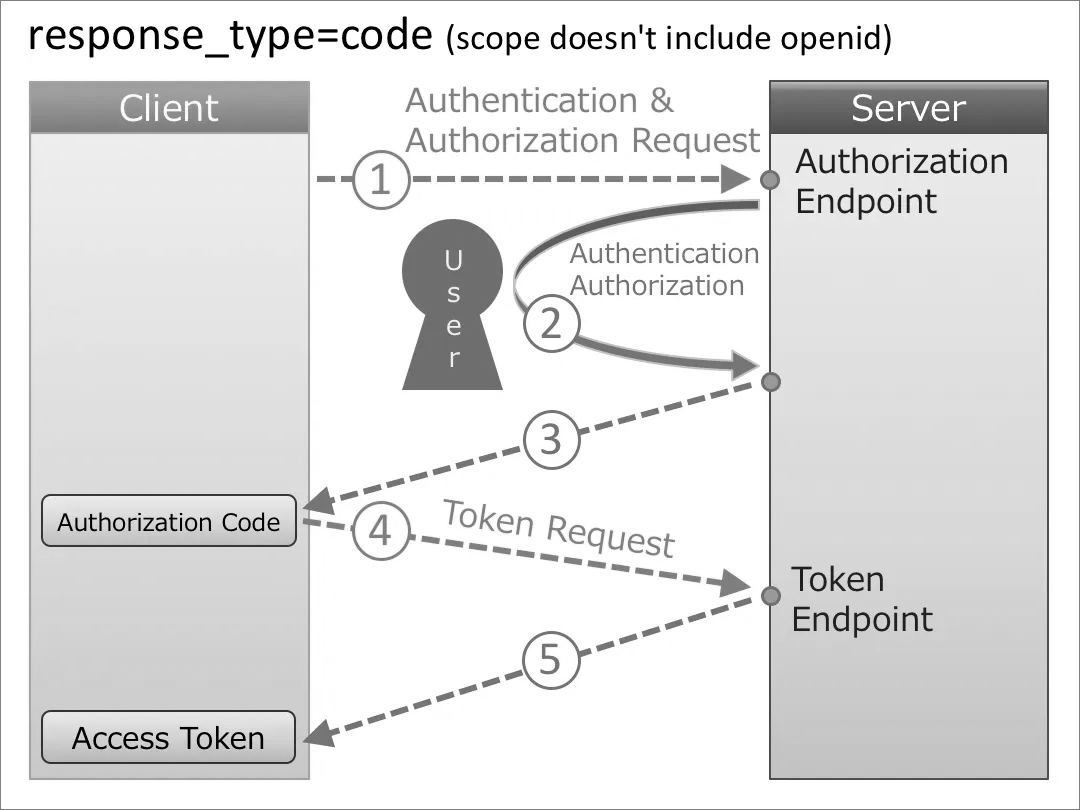
\includegraphics{images/png/oauth.png}}

    \fonte{\citeonline{OAuthImage2024}}
    \label{fig:oauth}
\end{figure}


\begin{enumerate}
    
    \item O serviço Web (Cliente) redireciona o utilizador para a tela de login no Servidor de Autorização, fornecendo seu identificador, \texttt{client\_id}.
    
    \item O indivíduo autentica-se perante o Servidor de Autorização e concede acesso ao seu recurso para o aplicação.
    
    \item O Servidor de Autorização emite o Código de autorização, que é encaminhado ao cliente via redirecionamento no navegador do usuário.
    
    \item A aplicação solicita o token de acesso correspondente ao seu código de autorização para o Servidor de Autorização. 
    
    \item O Servidor de Autorização encaminha o código de acesso. Nesse ponto, a troca é feita diretamente entre o backend da aplicação e o Servidor de Autorização, sem passar pelo navegador do usuário.

\end{enumerate}

Ao final do fluxo, a aplicação cliente utiliza o Token de Acesso para realizar requisições ao Servidor de Recursos, sendo autorizada a acessar apenas os recursos específicos concedidos pelo usuário. 

\subsection{OpenID Connect}\label{subsec:OIDC}

\sigla{OIDC}{OpenID Connect} é um protocolo de autenticação baseado na família de especificações OAuth 2.0, permitindo que as aplicações autentiquem usuários e obtenham informações sobre eles, proporcionando uma experiência de \acs{SSO} \cite{openid}. Ele é amplamente adotado por grandes provedores de identidade, como Google, Microsoft e Facebook, proporcionando uma interoperabilidade robusta e simplificada entre diversas plataformas e serviços, facilitando a integração e melhorando a segurança na autenticação de usuários em aplicações web e móveis.

Um novo token é definido chamado de \texttt{id\_token} para identificar os usuários para a aplicação. Este token está organizado em uma estrutura de \sigla{JWT}{JSON Web Token} que contém informações sobre a autenticação do usuário, incluindo o emissor do token, o público-alvo representado por um \texttt{client\_id}, um identificador único do usuário final no IdP, a data e hora da autenticação e os tempos de emissão e expiração do token. Para emitir esse token, novos fluxos também são definidos estendendo a especificação do parâmetro \texttt{response\_type}. No OAuth o valor de \texttt{response\_type} é code ou token. O \acs{OIDC} adiciona o \texttt{id\_token}, e permite qualquer combinação de code, token e \texttt{id\_token}. Um valor especial, none, também é adicionado. 

Também é adicionado o valor \textbf{openid} para o parâmetro \texttt{scope}, que é utilizado para definir as permissões específicas que uma aplicação está solicitando em relação aos dados do usuário. Especificamente, este valor permite que a aplicação obtenha um \texttt{id\_token}, que contém informações autenticadas sobre o usuário, como seu identificador único, e possivelmente outras informações adicionais se escopos adicionais como profile, email ou address forem incluídos. O escopo profile permite que a aplicação acesse uma variedade de informações de perfil básicas sobre o usuário. Isso pode incluir o nome completo, apelido, foto de perfil, gênero, data de nascimento, idioma preferido e outras informações de perfil. A inclusão deste escopo proporciona uma visão mais completa do usuário. O escopo email concede à aplicação acesso ao endereço de e-mail do usuário e a verificação se o endereço de e-mail foi verificado. Especificamente, a aplicação pode obter o endereço de e-mail e um indicador booleano (email\_verified) que informa se o endereço foi verificado. Isso é útil para aplicações que necessitam de um contato confiável com o usuário ou para validação de identidade. O escopo address permite que a aplicação acesse o endereço físico do usuário. Isso pode incluir informações como a rua, cidade, estado, código postal e país. A inclusão deste escopo é útil para aplicações que requerem informações de envio ou para personalizar ofertas e serviços baseados na localização do usuário.

Ademais, também é exigido a obrigatoriedade do \texttt{redirect\_uri} como medida de segurança para garantir que as Respostas da Autorização sejam enviadas apenas para URLs previamente autorizados. Isso ajuda a prevenir ataques como a homem no meio (man-in-the-middle) e a ataque de redirecionamento, onde um atacante poderia tentar interceptar ou redirecionar as respostas de autorização para um local malicioso. 

A \autoref{fig:openid}, descrita a seguir, demonstra o funcionamento do Fluxo de Código de Autorização no conxtexto do \acs{OIDC}. Nesse fluxo, ocorre a obtenção de um Código de Autorização, que é subsequentemente trocado por um \texttt{id\_token}.
Semelhante ao OAuth 2.0, após o usuário selecionar o \acs{IdP} de sua preferência, como o Google, ele é redirecionado pelo navegador por meio de uma requisição realizada pelo \acs{SP} (Cliente). A partir desse ponto, o fluxo descrito na imagem se inicia.

% Figura com o funcionamento do OIDC

\begin{figure}[htb]
    \caption{Fluxo de Código de Autorização no OIDC.}
    \centering
    \resizebox{0.5\linewidth}{!}{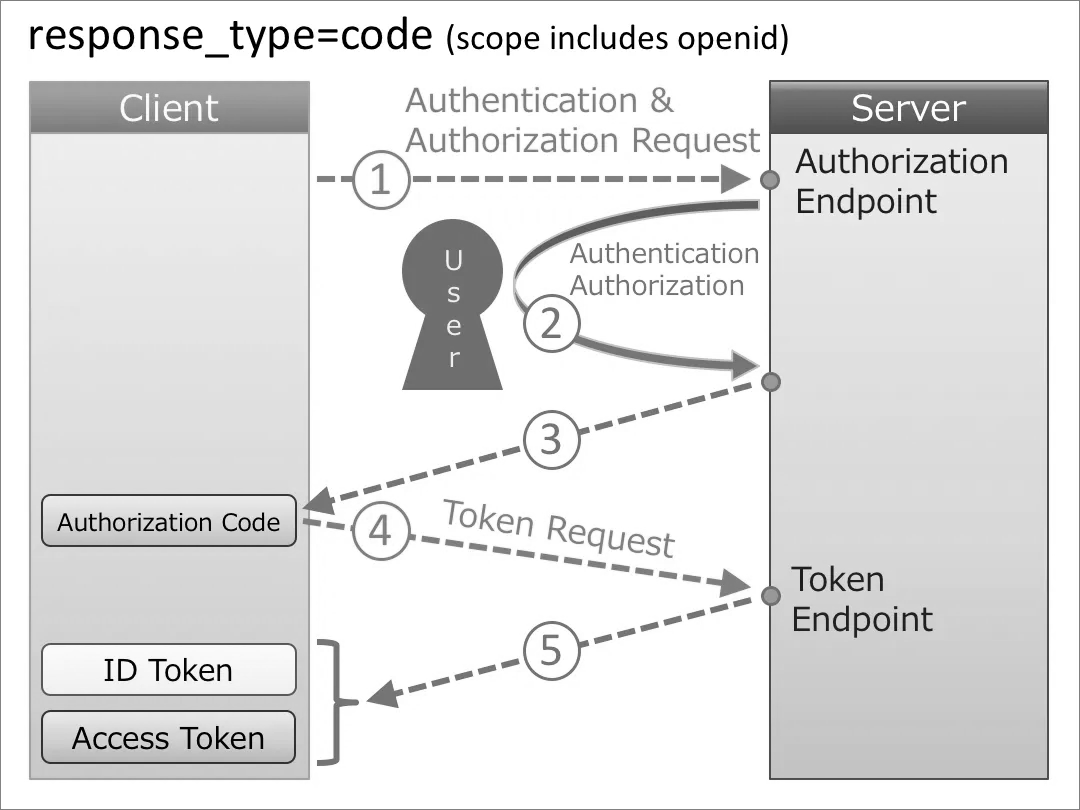
\includegraphics{images/png/openid.png}}
    \label{fig:openid}
    \fonte{\citeonline{OpendIDImage2024}}
\end{figure}


\begin{enumerate}
    
    \item O serviço Web (Cliente) redireciona o utilizador para a tela de login no Servidor de Autorização, fornecendo seu identificador, \texttt{client\_id}.
    
    \item O indivíduo autentica-se perante o Servidor de Autorização, fornecendo suas credenciais de acesso, como nome de usuário e senha.
    
    \item O Servidor de Autorização emite o Código de autorização, que é encaminhado ao cliente via redirecionamento no navegador do usuário.
    
    \item A aplicação solicita o token de acesso correspondente ao seu código de autorização para o Servidor de Autorização. 
    
    \item O Servidor de Autorização encaminha o código de acesso e o \texttt{id\_token}. Nesse ponto, a troca é feita diretamente entre o backend da aplicação e o Servidor de Autorização, sem passar pelo navegador do usuário.

\end{enumerate}

Ao final do fluxo, a aplicação cliente pode utilizar o \emph{UserInfo Endpoint} para obter informações adicionais sobre o usuário, como nome, e-mail ou outros dados, utilizando o código de acesso recebido. Após essa etapa, o usuário é autenticado com sucesso e redirecionado para a página do serviço, onde tem acesso aos recursos autorizados de acordo com seu perfil.

\subsection{OIDC4VC: O OpenID Connect no modelo SSI }\label{subsec:oidc4vc}

O \sigla{OIDC4VC}{OpenID Connect com Credenciais Verificáveis} representa um conjunto de protocolos avançados projetados para estabelecer um ecossistema de \acs{SSI} \cite{OIDC4VCWhitepaper2022}. Esse sistema capitaliza as funcionalidades robustas e amplamente validadas do OpenID Connect, amplamente adotado no modelo terceirizado de autenticação, oferecendo uma experiência segura e eficiente para a gestão de identidades digitais. Ao integrar Credenciais Verificáveis e, consequentemente, Apresentações Verificáveis ao \acs{OIDC}, o \acs{OIDC4VC} proporciona um mecanismo poderoso e flexível, permitindo que os indivíduos autentiquem e compartilhem suas identidades com uma combinação de segurança, privacidade e conveniência.  Essa abordagem garante que apenas os dados estritamente necessários sejam compartilhados em cada transação, oferecendo aos usuários um controle refinado sobre suas interações digitais.

O problema do protocolo \acs{OIDC} dentro do modelo Terceirizado é que ele levanta preocupações significativas sobre a redução de privacidade causada pela centralização de controle de credencias e a dificuldade de gerenciamento das mesmas em diferentes provedores. Durante o processo de autenticação usando o \acs{OIDC}, informações sensíveis sobre o indivíduo podem ser inadvertidamente compartilhadas com o \acs{IdP} que atua como Servidor de Autorização, como detalhes sobre quais serviços online a pessoa acessa \cite[Página 7]{OIDC4VCWhitepaper2022}. Isso ocorre porque a sua arquitetura centralizada concentra o controle das identidades digitais no \acs{IdP} (Servidor de Autorização).

Cada provedor emite e gerencia suas próprias credenciais de forma isolada, o que impede a unificação ou combinação de atributos provenientes de diferentes fontes em uma única credencial ou token. Por exemplo, um usuário pode ter uma credencial emitida por um banco que contém informações financeiras e outra credencial emitida por uma rede social com dados pessoais. No modelo \acs{OIDC}, esses atributos permanecem separados, e o usuário não tem uma maneira eficiente de combiná-los em um único artefato que possa ser utilizado para uma verificação mais simplificada de sua identidade em diversos contextos. Essa limitação não apenas aumenta a complexidade do gerenciamento de identidades, mas também restringe a flexibilidade e a utilidade das credenciais digitais, dificultando a criação de experiências de usuário mais integradas e seguras.

O \acs{OIDC4VC} visa abordar esses desafios de maneira eficaz, especialmente ao redefinir a responsabilidade do envolvida na emissão, armazenamento e apresentação das credenciais. Ao restringir o papel de \acs{IdP} a apenas emitir e delegar aos usuários a tarefa de armazenar e apresentar suas credenciais por meio de carteiras digitais, o novo ecossistema permite que os indivíduos exerçam um controle mais rigoroso sobre suas informações pessoais. Essa mudança possibilita que os usuários compartilhem seus dados diretamente com os serviços, de acordo com suas necessidades, garantindo que apenas as informações estritamente necessárias sejam divulgadas no momento oportuno. Essa abordagem fortalece a autonomia do usuário e promove um ambiente mais seguro e privado para a gestão de identidades digitais.

Ao empregar \acs{VP}s, os protocolos mitigam o problema da fragmentação das credenciais emitidas por diferentes provedores, possibilitando a unificação e combinação de atributos em um único artefato digital. Essa abordagem permite que o usuário consolide informações derivadas de múltiplas credenciais emitidas por diversas fontes, como exemplificado pela integração de dados provenientes de um banco e de uma rede social em uma única \acs{VP}. Dessa forma, o usuário pode fornecer, em suas interações com serviços online, uma representação mais completa e integrada de sua identidade. As \acs{VP} aprimoram o gerenciamento de identidades ao permitir que o usuário selecione e combine apenas os atributos necessários para cada contexto específico, promovendo uma experiência mais fluida e segura, ao mesmo tempo em que preservam a privacidade e mantêm o controle sobre as informações compartilhadas.

\subsubsection{Ecossistema}\label{subsubsection:ecossistema-oidc4vc}

Para sustentar essa estrutura, o \acs{OIDC4VC} estabelece uma série de protocolos e extensões que integram as funcionalidades do OpenID Connect ao modelo de Credenciais Verificáveis, conforme ilustrado na  \autoref{fig:protocol-opid4vc}.

% Figura com os três protocolos do OIDC4VC
\begin{figure}[htb]
    \caption{Ecossistema do OIDC4VC.}
    \centering
    
    \resizebox{\linewidth}{!}{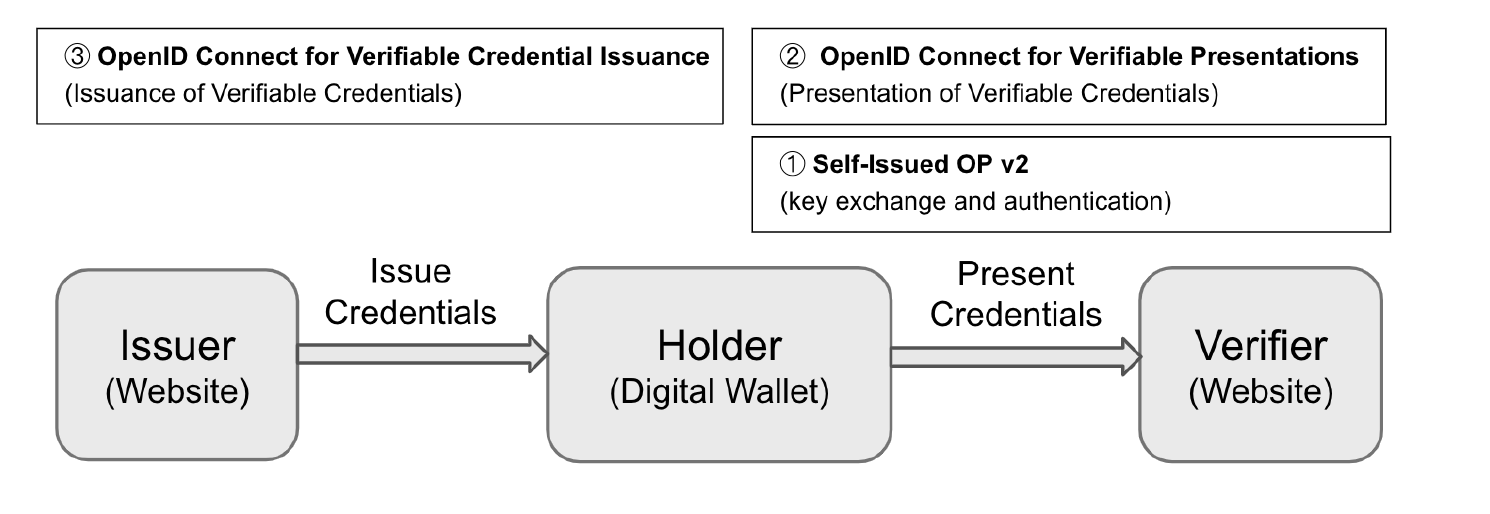
\includegraphics{images/png/protocol-of-OID4VC.png}}
    
    \label{fig:protocol-opid4vc}
    \fonte{\citeonline{OIDC4VCWhitepaper2022}}
\end{figure}


\begin{enumerate}

    \item \textbf{\sigla{SIOPv2}{Self-Issued OpenID Provider v2}}: É uma especificação que permite aos usuários atuarem como seus próprios \acs{IdP}, emitindo e gerenciando suas credenciais diretamente sem depender de um provedor de identidade terceirizado. Com ele o usuário pode gerar e assinar atributos como nome, e-mail, sem que sejam verificadas por uma entidade central. Além de conseguir provar que realmente controla a chave privada associada a essa assinatura (prova de posse) \cite{SIOPv2023}. 

    O \acs{SIOPv2} permite uma ampla variedade de arquiteturas de carteiras. Por exemplo, as carteiras podem ser executadas no dispositivo do usuário, mas também podem ser hospedadas na nuvem. A experiência do usuário pode ser fornecida por meio de um aplicativo móvel ou uma aplicação web. Do ponto de vista do protocolo, elas podem utilizar todos os fluxos do OpenID Connect, ou seja, há uma grande variedade de opções para atender às necessidades da respectiva implantação e dos casos de uso.
    
    \item \textbf{\sigla{OIDC4VP}{OpenID para Apresentações Verificáveis}}: Extensão do OpenID Connect para permitir os serviços solicitarem e receberem Apresentações Verificáveis \cite{OIDC4VP2023}.
    
    \item \textbf{\sigla{OIDC4CI}{OpenID para Emissão de Credenciais Verificáveis}}: Esta especificação propõe uma API destinada à emissão de \acs{VC}s em diversos formatos, incluindo o do W3C \cite{data-model-w3c}. As \acs{VC}s são emitidas por meio de uma carteira digital, previamente autorizada pelo usuário através do protocolo OAuth 2.0. Essa abordagem visa aproveitar as características comprovadas de segurança, simplicidade e flexibilidade inerentes ao protocolo OAuth 2.0 \cite{OIDC4CI2023}.

    Embora seja viável autorizar a emissão de credenciais conforme os serviços acessados requeiram informações do usuário, como ocorre no modelo terceirizado atual, a proposta das carteiras digitais visa proporcionar um maior controle ao usuário. Nesse modelo, os usuários armazenarão suas credenciais e gerarão \acs{VP}s individualizadas para cada serviço utilizado, o que reduz significativamente a possibilidade de os \acs{IdP}s monitorarem quais serviços são acessados e com que frequência isso ocorre.
    
\end{enumerate}

\subsubsection{OIDC4VP}\label{subsubsection:oidc4vp}

\acs{OIDC4VP} amplia as capacidades do OpenID ao permitir a apresentação de Credenciais Verificáveis na forma de Apresentações Verificáveis. Essa extensão oferece uma série de funcionalidades que reforçam a flexibilidade e a interoperabilidade do sistema, como a compatibilidade com todos os fluxos do OpenID Connect, o suporte a diferentes formatos de \acs{VC}s e \acs{VP}s, a capacidade de utilizar múltiplos métodos de transporte e o reaproveitamento do parâmetro claims para definir a sintaxe de solicitações. Nos parágrafos subsequentes, será detalhado cada um desses itens para fornecer uma compreensão mais profunda de suas funcionalidades e benefícios.

O protocolo é projetado para ser compatível com todos os fluxos do OpenID Connect. Isso significa que, independentemente do fluxo de autenticação escolhido, desde aqueles mais comuns como o Fluxo de Código de Autorização até naqueles em que o usuário é seu próprio provedor de identidade (\acs{SIOPv2}), \acs{OIDC4VP} pode ser integrado de maneira eficaz, garantindo flexibilidade e interoperabilidade.  Ademais, a sintaxe das solicitações reaproveita o parâmetro claims do \acs{OIDC} e utiliza a especificação DIF Presentation Exchange \cite{presentation-exchange} para formatar \acs{VP}s. 

O sistema oferece suporte a diferentes formatos de credenciais e apresentações, permitindo codificações em \sigla{JSON}{JavaScript Object Notation} ou \sigla{JSON-LD}{JSON for Linked Data}, bem como assinaturas utilizando \sigla{JWS}{JSON Web Signature} ou Linked Data Proofs. A capacidade de operar com diversos formatos e métodos de assinatura amplia significativamente a interoperabilidade do sistema, facilitando sua adaptação a diferentes padrões e requisitos técnicos. Por exemplo, o \acs{JSON} é amplamente utilizado em diversas aplicações web devido à sua simplicidade e eficiência \cite{JSONrfc82592017}, enquanto o \acs{JSON-LD} é preferido em contextos que demandam maior semântica e interconectividade de dados \cite{jsonld112020}. A escolha de formato é uma característica importante, porque determina se uma credencial suporta propriedades que reduzem a exposição de dados \cite{OIDC4CI2023Authlete}, como a Divulgação Seletiva e \acs{ZKP} descritas na \autoref{subsection:auto-soberano}.

A flexibilidade robusta na transmissão de \acs{VC}s e \acs{VP}s, suportando múltiplos métodos de transporte, é uma característica essencial. As informações podem ser integradas diretamente no \texttt{id\_token} ou na resposta do Userinfo, permitindo uma integração transparente com os fluxos de autenticação já existentes. Alternativamente, as credenciais podem ser transmitidas por meio de um token dedicado, o \textbf{\texttt{redirect\_uri}}, que pode ser retornado juntamente com o \texttt{id\_token} a partir dos endpoints de autorização ou token. Independentemente da forma que essa \acs{VP} seja encaminhada, para que a carteira saiba quais atributos são necessários, dentro da Requisição de Autorização, é reutilizado o parâmetro claims do \acs{OIDC} para conter um \texttt{redirect\_uri} com um \textbf{presentation\_definition}. Esse último contém uma \sigla{DA}{Definição de Apresentação} \cite{presentation-exchange}, que é uma estrutura que define como as apresentações devem ser enviadas para o \acs{SP}.


\subsubsection{Funcionamento}{\label{subsubsection:oidc4vc}}

No contexto desta especificação, a Carteira desempenha a função de Servidor de Autorização OAuth 2.0 em relação ao \acs{SP}, que, por sua vez, atua como Cliente OAuth 2.0 \cite{OIDC4VP2023}. Essa distinção é significativa, pois, em outras especificações, como no \acs{OIDC4CI}, a Carteira assume o papel de Cliente OAuth 2.0. Ademais, com essa definição, os \acs{SP} podem usufruir dos mecanismos existentes para facilitar o registro de clientes, como especificado no \sigla{OIDC-D}{OpenID Connect Discovery} \cite{sakimura2023openidDiscovery} e \sigla{OIDC-DCR}{OpenID Connect Dynamic Client Registration} \cite{sakimura2023openid-dcr}

As especificações \acs{OIDC-D} e \acs{OIDC-DCR} desempenham papéis complementares no ecossistema de autenticação do OpenID Connect. O \acs{OIDC-D} possibilita que os clientes descubram automaticamente as configurações e endpoints do provedor de identidade por meio de um documento de descoberta, facilitando a configuração e integração com o sistema de autenticação. Já o OIDC Dynamic Client Registration permite que clientes sejam registrados de forma dinâmica e automática com o provedor de identidade, sem a necessidade de intervenção manual, o que é particularmente útil em ambientes com alta demanda de novos clientes. Juntas, essas especificações tornam a gestão de autenticação e autorização mais ágil, flexível e escalável.

O funcionamento desse protocolo é estruturado em dois fluxos distintos. O primeiro, denominado \textbf{same-device flow}, refere-se ao processo no qual o usuário apresenta uma credencial a um \acs{SP} utilizando o mesmo dispositivo em que sua carteira digital está instalada. Nesse fluxo, tanto o \acs{SP} quanto a Carteira interagem diretamente no dispositivo do usuário, empregando redirecionamentos simples para a troca da Solicitação de Autorização (Authorization Request) e da Resposta de Autorização (Authorization Response) entre ambas as partes. Esse fluxo é exemplificado na figura \autoref{fig:samedevice}. O segundo fluxo, conhecido como \textbf{cross-device flow}, ocorre quando o \acs{SP} e a Carteira residem em dispositivos distintos. Nesse contexto, o \acs{SP} gera uma Solicitação de Autorização e a apresenta ao usuário na forma de um código QR (QR Code). O usuário, então, utiliza a Carteira em seu dispositivo para escanear o código QR e iniciar o processo de verificação, permitindo a continuidade da interação de forma segura e eficiente.

O protocolo introduz novos tipos de resposta (\texttt{response\_type}) para suportar a transmissão de tokens de apresentação verificável (\texttt{vp\_token}) em diferentes cenários de autenticação. Quando o valor de \texttt{response\_type} é \texttt{vp\_token}, a \acs{VP} é retornada diretamente na Resposta de Autorização (Authorization Response). No caso em que o valor de \texttt{response\_type} é \texttt{redirect\_uri} \texttt{id\_token} e o parâmetro \texttt{scope} contém \texttt{openid}, o \texttt{redirect\_uri} é retornado na Resposta de Autorização juntamente com um ID Token autoemitido, conforme definido no \cite{SIOPv2023}. Além disso, quando o \texttt{response\_type} é \textbf{code}, seguindo o Fluxo de Código de Autorização, o \texttt{redirect\_uri} é fornecido na Resposta de Token (Token Response), após a troca bem-sucedida do código de autorização pelo token correspondente. Nesse exemplo, o \texttt{response\_type} é \texttt{redirect\_uri}.

\begin{figure}[htb]
    \caption{Fluxo com Carteira e \acs{SP} no mesmo dispositivo}
    \centering
    
    \resizebox{\linewidth}{!}{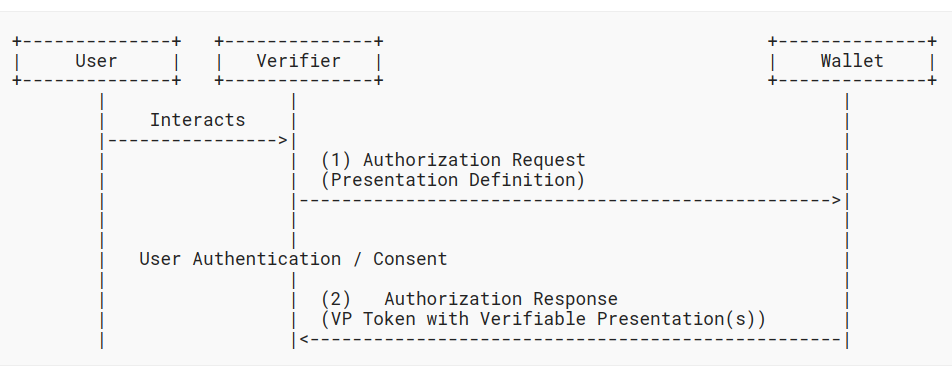
\includegraphics{images/png/same-device.png}}
    
    \label{fig:samedevice}
    \fonte{\citeonline{OIDC4VP2023}}
\end{figure}

\begin{enumerate}

    \item O \acs{SP} representado por um verficador, realiza um \textbf{Solicitação de Autorização} (Authorization Request) no \textbf{Endpoint de Autorização} para a carteira digital. 
    Nesse caso, o parâmetro \texttt{response\_type} inclui o valor \texttt{vp\_token}, enquanto o \texttt{presentation\_definition} contém a \acs{DA} que define os critérios que as \acs{VP}s devem cumprir, como o tipo de credencial exigido, o formato de apresentação e os atributos específicos das credenciais que devem ser compartilhados.    % Nesse caso, \texttt{response\_type} contém \texttt{redirect\_uri} e o \texttt{presentation\_definition} com a \acs{DA} com quais requisitos as \acs{VP}s devem cumprir, como o tipo de credencial utilizada, o formato em que devem ser apresentadas, quais atributos individuais dentro dessas credenciais devem ser apresentados. 
    
    \item A Carteira retorna a Resposta de Autorização, \emph{Authorization Response}. Nesse caso, com o \texttt{response\_type} definido como \texttt{vp\_token}, o valor de \texttt{vp\_token} é enviado diretamente.

    O \acs{SP} realiza a verificação da vinculação do titular (holder binding), bem como da integridade e autenticidade da credencial antes de seu processamento. Os procedimentos específicos a serem adotados variam conforme o formato da credencial, o esquema criptográfico utilizado e o mecanismo de revogação empregado, os quais estão além do escopo definido pelo \acs{OIDC4VP} \cite{OIDC4VCWhitepaper2022}.

\end{enumerate}

\newpage
\section{Análise formal de segurança}

A análise formal de segurança é um processo sistemático utilizado para garantir que protocolos atendam a requisitos de segurança específicos. O objetivo é verificar, de maneira matemática ou lógica, que um sistema se comporta corretamente \cite{Kulik2020}. Diferente das abordagens empíricas, como testes de penetração, que se concentram em identificar vulnerabilidades conhecidas, a análise formal permite detectar vulnerabilidades anteriormente desconhecidas, proporcionando uma garantia de segurança significativamente superior \cite{hauck2023openid}. Isso ocorre porque, enquanto os testes empíricos são limitados a cenários e ameaças específicas, a análise considera o comportamento completo do sistema, baseando-se em provas rigorosas, oferecendo uma segurança mais abrangente e fundamentada em teorias robustas.

A análise envolve três etapas, ilustrado na \autoref{fig:formal-analysis-steps}. A primeira é a \textbf{modelagem}, que consiste em criar uma representação abstrata do sistema, descrevendo suas operações, interações e comportamentos possíveis. A segunda é a \textbf{especificação de propriedades} em que são definidas, de forma precisa, as propriedades que o sistema deve atender em um contexto específico, como "um atacante não pode se autenticar como um usuário legítimo". Por fim, as \textbf{provas} que garantem que o modelo formal respeite as especificações de segurança definidas.

\begin{figure}[htb]
    \caption{Etapas da Análise Formal de Segurança.}
    \centering
    
    \resizebox{0.8\linewidth}{!}{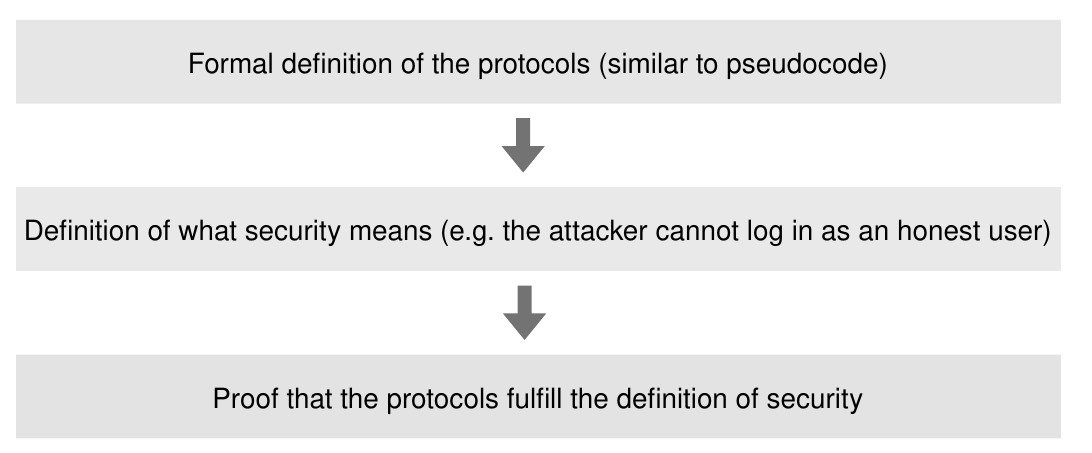
\includegraphics{images/png/formal-analysis-steps.png}}

    \fonte{\citeonline{hauck2023openid}}
    \label{fig:formal-analysis-steps}
\end{figure}


Para ilustrar o funcionamento desse tipo de análise, será reproduzida uma parte da Prova de Autenticação de Apresentação (Presentation Authentication) conforme descrita em \cite{hauck2023openid}. O objetivo deste capítulo não é fornecer uma explicação detalhada e exaustiva da prova, mas sim uma compreensão intuitiva do processo de análise. Este capítulo é, portanto, dividido em três subseções. Na \autoref{subsection:formal-definition-using-win}, será apresentado \sigla{WIM}{Web Infrastructure Model} utilizado como base para definir formalmente o \acs{OIDC4VP}, em um formato similar a pseudo-código. Na \autoref{subsection:properties-of-formal-analysis} será especificado o significado da Autenticação de Apresentação neste contexto, e, finalmente, na \autoref{subsection:proof-of-formal-analysis}, será apresentada a prova.

\subsection{Definição Formal de Protocolos Usando WIM}\label{subsection:formal-definition-using-win}

O modelo \acs{WIM} segue uma abordagem baseada no modelo \sigla{DV}{Dolev-Yao}, capturando padrões web amplamente utilizados, como HTTP e HTML. A \autoref{fig:wim-model} ilustra a arquitetura do modelo. Nele, cada entidade é representada por um processo que monitora um ou mais endereços IP e processa eventos correspondentes. Um evento é composto por uma mensagem e pelos endereços IP do remetente e do destinatário. Em cada etapa de processamento, um evento é selecionado de maneira não determinística de uma lista de eventos e entregue ao processo apropriado. A entidade processa o evento e gera um ou mais novos eventos, que são, então, adicionados à lista para processamento subsequente \cite{fett2024wim}.

Para modelar o \acs{OIDC4VP}, o comportamento do atacante e do navegador web são especificados como processos. 
O processo do atacante é um processo Dolev-Yao não determinístico que registra todas as mensagens que recebe e gera todos os eventos que pode derivar das mensagens registradas. 
Mais formalmente, um processo atacante $(I, Z, R, s_0)$ que recebe um evento de entrada $e_{in}$ em um estado $s$ gera o novo estado $s' = \langle e_{in}, E_{out}, s \rangle$ e os eventos 
$E_{out} = \{ \langle a_1, f_1, m_1 \rangle, \ldots, \langle a_n, f_n, m_n \rangle \}$ 
para algum $n \geq 0$, onde os endereços do remetente $f_1, \ldots, f_n$ são escolhidos de forma não determinística a partir de $I$, os endereços do destinatário $a_1, \ldots, a_n$ são escolhidos não deterministicamente entre todos os endereços IP, e as mensagens $m_1, \ldots, m_n$ são escolhidas não deterministicamente de $d(\{e_{in}\} \cup \{s\})$ \cite[Seção 2.5]{FettKS14}.
Dessa forma, um processo atacante é capaz de realizar todos os ataques que qualquer processo Dolev-Yao poderia executar, exceto quebrar criptografia.

Nesta análise, utiliza-se o modelo de atacante de rede, que tem acesso a todos os endereços IP, permitindo-lhe interceptar mensagens destinadas a outras partes e falsificar os endereços dos remetentes. Em redes reais, esses ataques podem incluir ARP-spoofing, onde o atacante redireciona tráfego em redes locais ao falsificar a correspondência entre endereços IP e endereços MAC, e ações de adversários patrocinados por estados-nação, que exploram infraestrutura de telecomunicação para interceptar e manipular dados em larga escala.

O atacante pode, ainda, corromper qualquer processo legítimo, ganhando acesso completo ao estado da entidade comprometida.
Isso é representado pelo envio de uma mensagem especial, $m = \text{CORRUPT}$, ao processo correspondente \cite[Seção 2.5]{FettKS14}. Após receber essa mensagem, o processo começa a atuar como um processo atacante, utilizando o último estado disponível. Os detalhes sobre como ocorre a corrupção variam de acordo com o modelo específico do processo.


O navegador web faz parte de um sistema que formaliza a infraestrutura da web e suas aplicações associadas. Para simplificar o modelo, o \acs{WIM} inclui um servidor HTTPS genérico, responsável, entre outras funções, por receber e enviar requisições HTTPS.

\begin{figure}[htb]
    \caption{Modelo WIM}
    \centering
    \resizebox{\linewidth}{!}{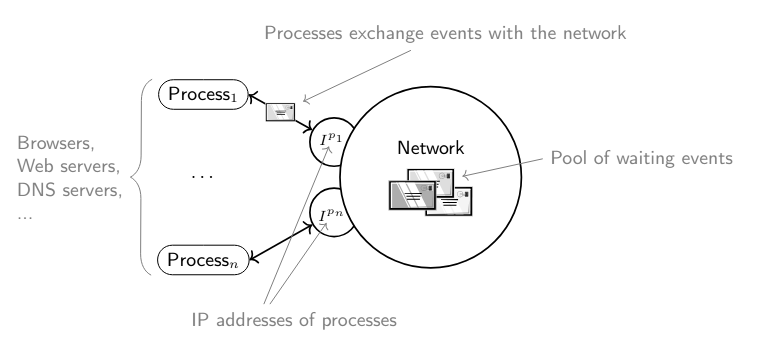
\includegraphics{images/png/wim-model.png}}
    \label{fig:wim-model}
    \fonte{\cite{fett2024wim}}
\end{figure}

\subsection{Propriedades de segurança}\label{subsection:properties-of-formal-analysis}


Uma etapa crucial para a comprovação de segurança é definir o que ela significa em um contexto específico, o que se faz por meio da identificação das propriedades de segurança relevantes. No caso do \acs{OIDC4VP}, uma dessas propriedades é a \textbf{Autenticação de Apresentação} (Presentation Authentication), que garante que um atacante não consiga se passar por um usuário legítimo para acessar uma aplicação. Em um ambiente web, essa propriedade é comprometida se um atacante obtiver posse de um cookie de sessão associado a um ID de usuário legítimo.

\subsection{Prova de segurança}\label{subsection:proof-of-formal-analysis}

% ---------------------- DECISÃO DE EXPLICAÇÃO ----------------------------------%
% - Não vou falar do response_mode direct_post. Teria que explicar mais um fluxo, e não acrescenta nada na proposta. Seria apenas ilustrativo para mostrar como a prova funciona.
% - Estou desconsiderando (Same-device e Cross-device flow), pois ao meu ver os tipos de ataques (Conseguir a apresentação e conseguir o session ID autorizado), servem tanto para um quanto para outro
% ---------------------- DECISÃO DE EXPLICAÇÃO ----------------------------------%

Para demonstrar a segurança da Autenticação de Apresentação, são estabelecidas duas premissas: (1) o usuário é perfeito, ou seja, ele sempre mantém o controle de quais fluxos iniciou; e (2) as entidades Browser, Carteira e Verificador são honestas, ou seja, não divulgam informações. Com base nessas premissas, deve-se provar que o atacante não consegue obter um cookie de sessão vinculado à identidade de um usuário legítimo. Isso ocorre porque as sessões são tipicamente identificadas por um nonce armazenado no navegador do usuário como um cookie. Se um atacante obtiver acesso a esse cookie, ele pode se passar pelo usuário legítimo, reutilizando o cookie comprometido para acessar a sessão ativa no sistema e, assim, obter os mesmos privilégios e acessos que o usuário original.

O cookie é gerado apenas no endpoint de redirecionamento (redirect endpoint), onde o verificador recebe a resposta de autorização (Authorization Response). Para que o atacante obtenha esse cookie, existem duas opções: a primeira seria que uma das partes honestas vazasse o cookie de sessão, o que é prevenido pela premissa (2); a segunda seria o atacante conseguir utilizar o redirect endpoint do verificador com sucesso. No entanto, isso só pode ser feito por meio de uma resposta de autorização contendo um \textbf{\texttt{redirect\_uri}}.


% \newtheorem{premise}{Premissa}
% \begin{premise}
%     \textbf{O usuário é perfeito}\label{premise:perfect-user}: O usuário sempre mantém o controle de quais fluxos ele iniciou.
% \end{premise}

% \begin{premise}
%     \textbf{As entidades Browser, Carteira e Verificador são honestas}\label{premise:honest-entity}: Entidades que não divulgam informações.
% \end{premise}

Para que o atacante obtenha um \textbf{\texttt{redirect\_uri}} com a identidade de um usuário legítimo, a possibilidade de uma entidade honesta divulgá-lo é descartada, conforme descrito em (1). Além disso, o atacante poderia tentar acessar a chave privada associada à chave pública da credencial do usuário, o que também é impedido pela \textbf{Propriedade de Emissão Autenticada}, detalhada em \cite{hauck2023openid}. Outra opção seria induzir uma carteira legítima a criar um \textbf{\texttt{redirect\_uri}} arbitrário.

Uma das táticas que o atacante pode usar para induzir uma carteira a gerar um \textbf{\texttt{redirect\_uri}} envolve o uso de um ataque de phishing. Nesse cenário, o atacante engana o usuário para que ele clique em um link ou visite uma página maliciosa, desencadeando involuntariamente um processo de autenticação com sua carteira digital. Durante esse processo, a carteira recebe uma requisição de autorização com o parâmetro \textbf{\texttt{redirect\_uri}} direcionado para um domínio controlado pelo atacante. No entanto, ao obter o \textbf{\texttt{redirect\_uri}}, o atacante não consegue utilizá-lo, pois o parâmetro \textbf{aud} (audience) é preenchido com o domínio do \textbf{\texttt{redirect\_uri}}, tornando o ataque ineficaz.


% ---------------------- DECISÃO DE EXPLICAÇÃO ----------------------------------%
% - Esse fluxo só acontece no response_mode direct_post. 
% ---------------------- DECISÃO DE EXPLICAÇÃO ----------------------------------%
% Um segundo cenário de ataque ocorre quando o atacante obtém conhecimento de um ID de Sessão previamente autenticado. Para que isso aconteça, seria necessário violar a(\autoref{premise:honest-entity}), que é uma garantia de segurança. No entanto, o atacante ainda pode tentar enganar o usuário. Nesse cenário, o atacante pode criar um ID de Sessão com um verificador e fazer o usuário enviar uma apresentação com as suas credenciais para a sessão iniciada pelo atacante. Isso não ocorrerá, desde que o usuário esteja ciente dos seus fluxos, como descrito pela garantia \autoref{premise:perfect-user}.

\begin{figure}[htb]
    \caption{Prova de Autenticação da Apresentação}
    \centering
    \resizebox{\linewidth}{!}{
        \begin{tikzpicture}[
    node distance=2cm and 3cm,
    every node/.style={draw, rectangle, align=center, text width=5cm, minimum height=2cm},
    arrow/.style={draw, -{Latex[width=2mm]}, thick}
    ]
    
    % Nodes
    \node (l1) {O atacante obtém o token de serviço};
    
    \node (l2-1) [below left=of l1] {O atacante consegue chamar o redirect\_endpoint com sucesso.};
    \node (l2-2) [below right=of l1] {Token de serviço é divulgado por meio de uma entidade honesta};
    
    \node (l3-1) [below left=of l2-1] {Atacante obtém um vp\_token válido};
    % \node (l3-2) [below right=of l2-1] {Atacante conhece um ID de sessão autorizada};
    \node (l3-3) [below=of l2-2, fill=gray!20] {\textbf{Falso}\\em virtude da Premissa 1};
    
    \node (l4-1) [below left=of l3-1] {O vp\_token é divulgado para o atacante};
    \node (l4-2) [below=of l3-1] {O atacante induz uma carteira legítima a gerar um vp\_token em seu nome, permitindo que ele o envie para um verificador.};
    \node (l4-3) [below right=of l3-1] {Atacante sabe a chave privada da credencial do usuário legítimo};
    % \node (l4-4) [below=of l3-2] {O atacante cria seu próprio ID de sessão com o verificador};
    % \node (l4-5) [below right=of l3-2] {ID de Sessão é divulgado};
    
    \node (l5-1) [below=of l4-1, fill=gray!20] {\textbf{Falso}\\em virtude da Premissa 1};
    % ---------------------- EXPLICAÇÃO ----------------------------------%
    % -- Existe a possibilidade de não alterar o redirect\_uri. Porém o atacante teria que:
    % -- 1. Fazer um script para iniciar a sessão com um verificador (Ter um ID de Sessão para o usuário mas que o atacante tenha acesso?)
    % -- 2.1 Atacante pode interceptar a resposta, mas está criptografada.
    % -- 2.2 A resposta chega e redireciona o usuário para o redirec_uri definido previamente (fluxo normal seguro)
    % -- OU
    % -- 1. O Atacante inicia uma sessão com um verificador fora do browser do usuário
    % -- 2. Engana o usuário (com um script no browser dele) para enviar o vp_token para o verificador que o atacante tem um ID de Sessão.
    % -- 3. Verificador recebe o vp_token, mas dá erro porque vem com a origem do usuário a qual não têm sessão com ele.
    % ---------------------- EXPLICAÇÃO ----------------------------------%
    \node (l5-2) [below=of l4-2] {O atacante tenta modificar a Requisição de Autorização enviada à carteira, alterando o \textbf{redirect\_uri} para um domínio sob seu controle, com o objetivo de redirecionar a resposta para um verificador legítimo e se passar pelo usuário que solicitou a apresentação.};
    \node (l5-3) [below=of l4-3, fill=gray!50] {\textbf{Falso}\\Quebra a Propriedade de segurança da autenticação de emissão};
    % \node (l5-4) [below=of l4-4] {A requisição de autorização é enviada ao usuário através de phishing};
    % \node (l5-5) [below=of l4-5, fill=gray!20] {\textbf{Falso}\\em virtude da Premissa 1};
    

    % ---------------------- EXPLICAÇÃO ----------------------------------%
    % - O nodo abaixo pode parecer incompleto, ou mal explicado, mas a jutificativa está diretamente relacionada com a proposta de algoritmo que está descrita no texto.


  
    % ----------------------  EXPLICAÇÃO ----------------------------------%
    \node (l6-1) [below=of l5-2, fill=gray!20]  {\textbf{Falso}\\O atacante não consegue gerar um vp\_token válido, pois o campo \textbf{aud} utiliza o domínio do \textbf{redirect\_uri} como valor, tornando-o inválido e inutilizável.};

    % \node (l6-2) [below=of l5-4, fill=gray!20] {\textbf{Falso}\\em virtude da Premissa 2};
    
    % Connections
    \draw[arrow] (l1) -- (l2-1);
    \draw[arrow] (l1) -- (l2-2);
    \draw[arrow] (l2-1) -- (l3-1);
    % \draw[arrow] (l2-1) -- (l3-2);
    \draw[arrow] (l2-2) -- (l3-3);
    \draw[arrow] (l3-1) -- (l4-1);
    \draw[arrow] (l3-1) -- (l4-2);
    \draw[arrow] (l3-1) -- (l4-3);
    % \draw[arrow] (l3-2) -- (l4-4);
    % \draw[arrow] (l3-2) -- (l4-5);
    \draw[arrow] (l4-1) -- (l5-1);
    \draw[arrow] (l4-2) -- (l5-2);
    \draw[arrow] (l4-3) -- (l5-3);
    % \draw[arrow] (l4-4) -- (l5-4);
    % \draw[arrow] (l4-5) -- (l5-5);
    % \draw[arrow] (l5-4) -- (l6-2);
    

    \draw[arrow] (l5-2) -- (l6-1);
   
    
\end{tikzpicture}

    }
    \fonte{O Autor}
    \label{fig:proof-of-presentation-authentication}
\end{figure}